\documentclass[conference]{IEEEtran}
\usepackage[noadjust]{cite}
\usepackage{amsmath}
\usepackage{notoccite}
\usepackage{algorithm}
\usepackage[noend]{algpseudocode}
\usepackage{graphicx}
\usepackage{subcaption} 
\usepackage{verbatimbox}
\usepackage{multirow}
\usepackage{pbox}
\usepackage{tabularx} 
\usepackage{adjustbox}
\usepackage{rotating}
\usepackage{epstopdf}
\usepackage[justification=centering]{caption}% or e.g. [format=hang]


\hyphenation{op-tical net-works semi-conduc-tor}    

\title{Continuous User Verification\\via Mouse Activities}

\begin{document}
\maketitle


\begin{abstract}
Behavioral biometrics such as mouse dynamics is gaining attention these days to address the limitations of
conventional verification systems. In this paper we present a novel method to continuously verify a system user via
his/her mouse activities. Our method, based on simple statistical profile, was tested using 45 users’ 76,500 mouse activities.
A total of 354,375 genuine and impostor verification attempts have been performed by deploying 175 different verifier
setups. In our experiments, we achieved an impressive low Equal Error Rate (EER) of 6.72\%. On average the EER
was 13.42\%. We opine that, our method can complement the regular verification systems and can serve better for
continuous verification purpose because of its simplicity.
\end{abstract}
\begin{IEEEkeywords} 
Mouse Dynamics,
Behavioral Biometrics,
Continuous Verification.
 \end{IEEEkeywords}
\IEEEpeerreviewmaketitle

\section{Introduction \& Background}


While relatively new, mouse dynamic user authentication does have existing research. The research already done, however, has limitations. The majority of the existing research was done with a relatively small population. Using a small population when conducting research can affect the results of that research. Larger sample sizes allow for more accurate results. Another limitation present in existing research is high false acceptance rates. When testing for authentication, the amount of false acceptances should be as close to 0\% as possible. Having both higher false acceptance rates and false rejection rates leaves room for improvement on the research conducted. Research regarding mouse dynamic user authentication that has seen high success rates is when the authentication is used as a login measure, for example, using the mouse to draw a pattern to log into a machine instead of typing in a password or scanning a fingerprint. There are limitations to this research as well, the biggest being that drawing a pattern with the mouse can easily be reproduced. Also, this form of authentication is performed once and the user is granted access, it does not continuously verify that user.

One significant limitation in existing mouse dynamic user authentication research is the high false acceptance rates and false rejection rates. High FAR and FRR percentages mean that the system has low accuracy when successfully rejecting or accepting a user. We see this occurring with multiple accounts of previous research done in this area \cite{Jor, CS, Sch}. One of these research procedures only took into account mouse curves when authenticating a user \cite{Sch}. This could be the reason they saw such high FAR and FRR rates, successful authentication is more difficult to achieve when only a few characteristics are used to build a user profile. In order to create a more practical and accurate system for mouse dynamic user authentication, FAR and FRR rates need to be significantly lower.

There has been some previous research done with very promising results. However, while this research saw false acceptance rates at only .43\% and false rejection rates at 1.75\%, the population size used was very low, they only used 11 subjects when conducting their research. While the results they achieved are more successful than the majority of other research done in this area, their low subject count raises questions about how reliable their system really is. When using a broader subject count, there is a possibility that these low FAR and FRR percentages would no longer be as low as originally recorded. It is hard to tell reliability when such a small population is being used. \cite{Pus} One study that saw very low FAR and FRR rates at 0.55\% and 3\% respectively, only used 10 subjects to calculate these results. These subjects were also studied over a long period time, making the system much more accurate. This method would be difficult to implement on a larger group of people to get results that accurate \cite{She}. Another instance where this research saw low FAR and FRR rates (just over 2\%) also had a relatively low subject count. This research used a slightly larger number of subjects, 22, but even that number is still relatively low to see accurate results for large populations of people. \cite{Ahmed}

Some promising research that has been done so far in this area used 37 subjects, saw relatively low FAR and FRR rates at slightly under 10\%, and used a fast authentication time at 11.8 seconds \cite{CS}. Even this research could see improvement though. While the FAR and FRR rates are lower than most other research with a fast authentication time, they are still higher than what is desired. If lower FAR and FRR rates could be achieved at an even faster authentication time, practicality of the system would increase. Another instance of promising results found in this area of research saw an equal error rate of 1.3\%. The researchers that conducted this research had an interesting point when discussing their results. They said that while their results were promising, they did not expect the results to stay as accurate if a larger sample size was used. They came to this conclusion based off of research done on keystroke dynamics, saying that larger sample sizes make chances of two users having similar characteristics increases significantly \cite{Zhe}.

The most promising existing mouse dynamic authentication research achieved false acceptance rates at 0\% and false rejection rates at 0.36\%. The results achieved in this research make it the first conducted on mouse dynamics as a continuous verification system to reach the European standard for access control, which is a FAR rate less than 0.001\% and a FRR rate less than 1\% \cite{Nak}.

One method of mouse authentication that has seen very promising and positive results is using the mouse as a login procedure. One research procedure had users use the mouse to login as if unlocking a combination lock. They saw successful results with low false rejection and false acceptance rates \cite{HJ}. Another research procedure had users draw a complex figure with the mouse to login. They saw a 93\% successful verification rate with their research \cite{Syu}. While the results of mouse authentication through the use of a mouse to draw a pattern to login into a system are promising, it is not as practical as a continuous verification system would be. Drawing a pattern with the mouse is more easily replicated than a user’s specific and unique everyday normal use of the mouse.   

Our research on mouse dynamic user authentication addresses the limitations talked about. We have used a larger population base to take our samples from to increase our accuracy. We are also working to achieve low false acceptance and false rejection rates. With our research, we have taken a larger variety of mouse characteristics into consideration when measuring the uniqueness of a user’s mouse characteristics. Using a larger amount of mouse characteristics can build a more complete and specific profile for each user. With more detailed user profiles, there is less likelihood for another user to create similar results and ultimately a false acceptance as another user. More detailed profiles also capture a more accurate representation of a user, which can also lower the amount of false rejection rates.


\begin{figure}[h!]
  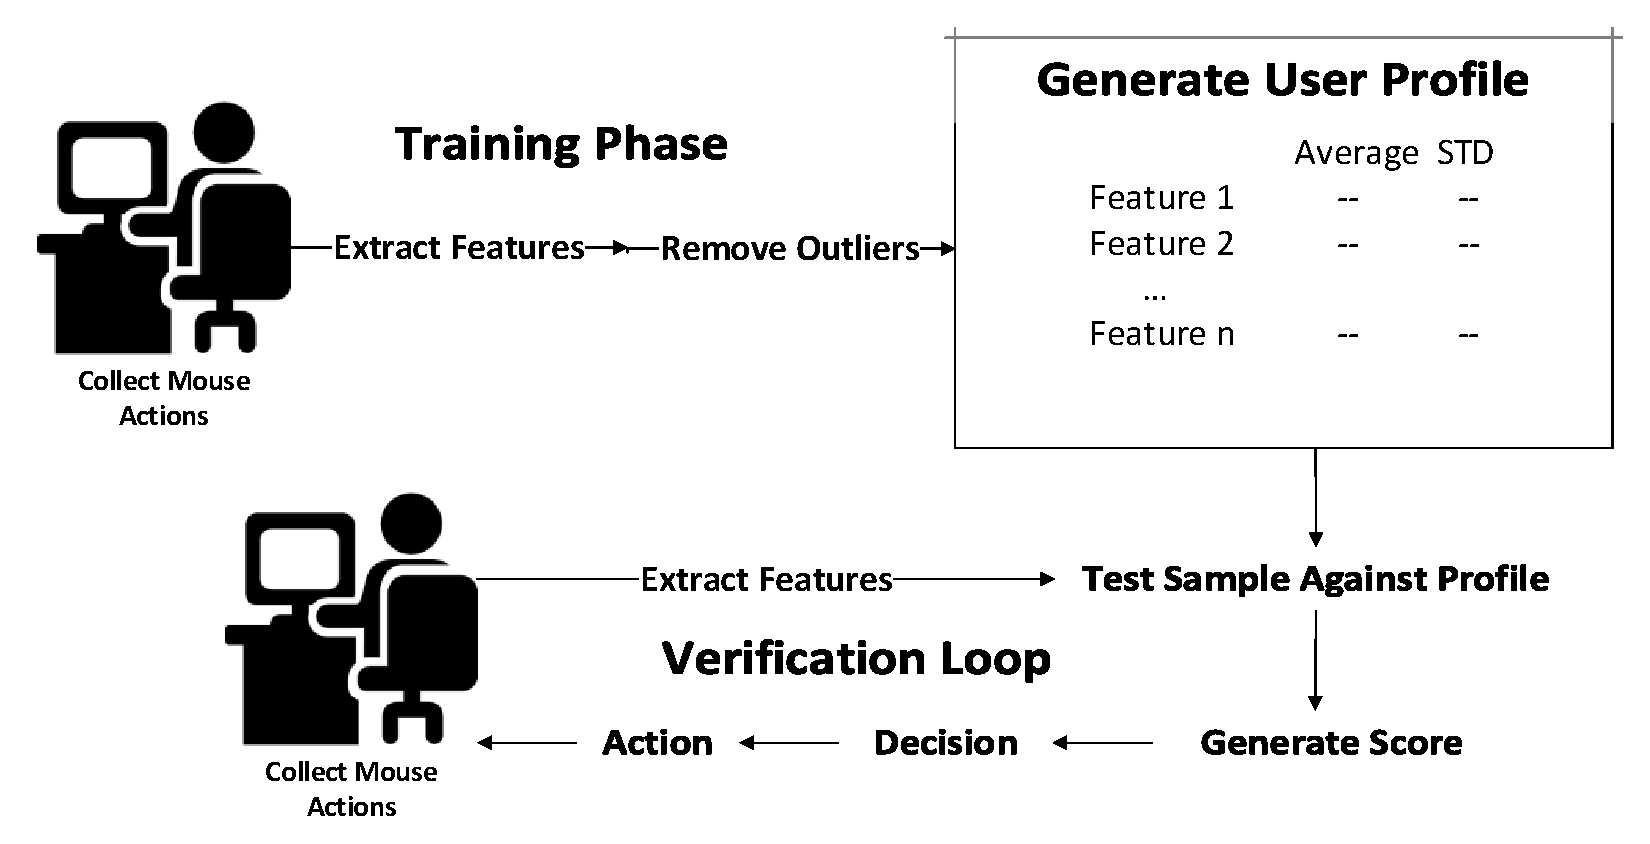
\includegraphics[width=1\linewidth]{Overview.pdf}
\caption{An overview of continuous verification with mouse movements. In the training phase a user creates a profile based on their mouse movements (The average and standard deviation of each mouse feature). The profile is used to represent a user in the verification phase where features from live mouse movements can be verified against the profile in order to determine if the live mouse movements came from the user who created the profile. If the verifier determines that the live mouse movements are illegitimate an action can be taken. ( e.g. logging the user out, creating a log of the incident, etc.)}
\end{figure}


\section{Data Collection}
We wanted our data set to include movements that were natural to best simulate day to day actions a user would perform on the computer in order to have a more relevant set of data to what our authenticator would see in a practical environment. To do this, we asked a class of students to record their mouse movements. The students were instructed to perform any activity on the computer they normally would for an hour period.  
	In order to log the mouse activity of users we created a simple mouse logger.  The logger was a small piece of software that ran on the windows operating system. The logger, when run on a machine, logged the position of the cursor using the windows method GetCursorPos(), the state of the left and right mouse buttons (up or down), and a timestamp every 15.6ms. 15.6ms being the default timer resolution that windows supports. The resulting log was then placed into a text file. 
We then screened the samples and removed samples with very few (0 to 10) movements and samples that weren't an hour long. Post-screening we had 25 valid user samples.  Our samples consisted of university students and their friends and family collected from late November to early December 2014.


\bgroup
\def\arraystretch{1.5}
\addvbuffer[12pt 8pt]{\begin{tabular}{l*{6}{c}r}
\textbf{Type}              &\textbf{ Maximum} & \textbf{Minimum} & \textbf{Average} \\
\hline
Left Clicks	& 716 & 37 & 547.84 \\
Right Clicks	& 690 & 0 & 122.8 \\
Double Clicks	& 1282 & 1 & 181.64 \\

\end{tabular}}
\egroup
\captionof{table}{Overview of the samples collected}


\section{Feature Extraction}
    In order to classify a test sample we needed some way to compare test samples and training samples. To do this we used features that are found in our definition of a mouse movement. The features, defined in Table \ref{tbl:definitions} and visualized in Figure \ref{fig:visualdefinition}, were found to be unique between users. In total we had 6 features. The double click length feature is interesting in that it contains 3 sub features allowing each sample to have a unique double click feature even if the entire length of the double clicks happen to be the same.
	We defined a mouse movement as a period of cursor movement followed by a click. This isn't to say that a click without any movement prior is not considered a mouse movement. It would be a mouse movement with no speed, acceleration, or jerk. If the cursor sustains no action for a period of 500ms or longer we classify that period as a pause to allow for periods where the user is not concentrating on moving the mouse or not moving it with conscious effort.

\bgroup
\def\arraystretch{1.5}
\begin{table*}
\begin{tabular}{m{.25\textwidth} | m{.75\textwidth}  }
\label{tbl:definitions}
 \textbf{ Feature}	&	\textbf{Description}\\
 \hline
 Single Left Click Length	&	\multirow{2}{*}{\pbox{20cm}{The length of a click from the first record the mouse button is found to be \\ down to the first record the mouse button is found to be up.}}\\
\cline{1-1}
 Single Right Click Length	&	\\
\hline
 Double Click Length	&	\pbox{20cm}{Split into 4 sub-features: Total Length and intervals 1,2, and 3.\\
Total length: The time between the first record the mouse is found to be down and the first record the mouse\\ is found to be up after the second click.\\
Interval 1: The first single left click length in a double click.\\
Interval 2: The time between the first record of the left mouse button being found up after the first click to the\\ first record of the left mouse button being found down for the second left click.\\
Interval 3: The second single left click length in a double click.}\\
\hline
 Speed			&	Distance the cursor travelled divided by the total time of the movement up until the click.\\
\hline
Acceleration			&	Change in Speed over time\\
\hline
Jerk				&	Change in Acceleration over time\\

\end{tabular}
\caption{Descriptions of the features used}
\end{table*}
\egroup




\section{Methodology}


\subsection{Outlier Filtering}
For our setup we first went through each of the user samples and extracted each of the features, as defined above, from each mouse movement. To remove rare cases of mouse movements where the user provides a mouse movement far from the mean we implemented an outlier removal scheme. We define a mouse feature to be an outlier if it is more eccentric than 66\% of the population of the same mouse features for a single user. For example, if we are looking to find if a particular mouse feature M is an outlier:

\begin{algorithm}

\caption{Determines if a single feature $F$ is an outlier from the rest of the population of its own kind. $featurePopulation$ is an array of same-typed features from a testing sample that $F$ is also a member of.}\label{euclid}
\begin{algorithmic}[1]
\Procedure{IsAnOutlier}{$F$}
\State $\textit{count} \gets 0$
	\For{\textbf{each} $feature \textrm{ in } featurePopulation$}
			\If{$ |F - feature| > R$}
				\State $count \gets count + 1$
			\EndIf
	\EndFor
	\If{$count \div featurePopulation_{size} \ge .33$}

		\State \Return{\texttt{True}}
	\Else
		\State \Return{\texttt{False}} 

	\EndIf
\EndProcedure
\end{algorithmic}
\label{alg:algorithm1}

\end{algorithm}

We defined the variable R, for each mouse feature, a number large enough to include most of the population while small enough to remove the noise from the data. We found optimal values for our R values after extensive experimentation we will describe later on.\\
We created a simple algorithm for determining if a particular record of a mouse feature is an outlier outlined in Algorithm \ref{alg:algorithm1}. For a given set of mouse features from a training sample (the featurePopulation), we compared each feature in the featurePopulation against every other feature of the same type, i.e. a Single Left Click Length feature is only compared to every other Single Left Click Length feature. Then a simple tally is kept of how many of the features in the featurePopulation have a distance greater than R as shown on line 4 \& 5 of Algorithm \ref{alg:algorithm1}. On line 6 we simple restate that if the if the tally is greater than 33\% of the featurePopulation we claim the feature F is an outlier and discard it from the training set.


\begin{figure}[t]
  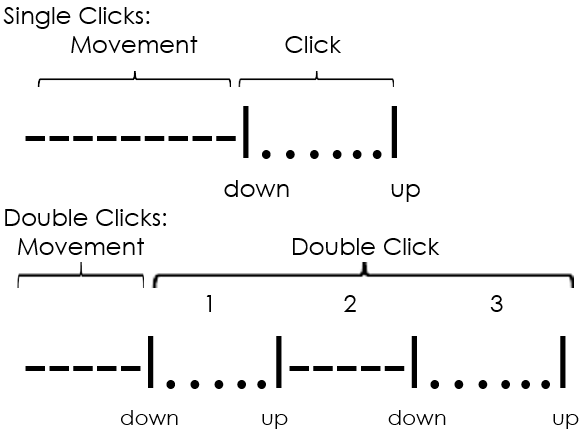
\includegraphics[width=1\linewidth]{clickDiag}
  \label{fig:visualdefinition}
  \caption{A visual representation of the click features. Dashes representing no button activity, dots representing periods where the mouse button is down, and vertical bars representing the first record that the mouse button has changed state.}
\end{figure}

\subsection{Verification}
	To authenticate a user based on their mouse movements we analyze six mouse features over the course of a sample. Our method is a simplistic user-authentication model. We create a profile based on a user's past behavior then test further samples against that profile to determine if the sample we test with is close enough to the previous profile to be considered the same user.  
We then split the edited list of features into a testing set and a training set. For each file we create user profiles based on half of the user's sample (about 50 mouse movements on average for our samples). The profiles being simply the averages and standard deviations of each of the mouse features. The mouse movements from the sample that we did not use for the profile go into the user's testing set.
Using a simple classification scoring method we can see how well a user profile and a testing set of data match up. For our entire set of data we took every user profile and tested each against every testing set. Our custom testing method generated a score for each test between 0 and 1. 1 being a perfect match and 0 being a perfect mismatch.
We tested by comparing each of the mouse movements in a testing set against the users profile. If the features in the mouse movement are within m standard deviations of the corresponding means in the user profile then the test gets a point. The total amount of points accrued is divided by the total amount of mouse movements in the file to generate the score.
	


\section{Experimental Setup}
We had a few parameters where it wasn’t immediately apparent how to set. For the R variables we needed values that can discriminate mouse feature values that are too eccentric while keeping as much unique data as possible. To solve this we ran a script that ran the tests and found the EER over an array of values for each parameter to determine the optimal values where the EER is at its lowest. We found that an M value of 1.9, a Single Click R of 15, and a Double Click R of 175 to produce the lowest EER for our set of data.

\bgroup
\def\arraystretch{1.5}
\addvbuffer[12pt 8pt]{\begin{tabular}{ l| l}
\textbf{Parameter}              &\textbf{ Values Tested} \\
\hline
Single Click R		& 15 20 25 30 25  \\
Double Click R	& 175 180 185 190 195\\
M Values		& 0.7 1 1.3 1.6 1.9 2.2 2.3\\
\end{tabular}}
\egroup
\captionof{table}{The values used for our parameters for testing. By varying the parameter value we experimented with 175 (5 Single Click R x 5 Double Click R x 7 M Values) different experimental set-ups. Note that we do not use any R parameter for the other features since they show less variance. In total, we experimented with 354,357 verification attempts (45 users x 45 users x 175 experimental set-ups).}



\section{Experimental Results \& Analysis}
To calculate the results of our experiment we took each users profile and tested that against every other set of testing data. This values in this generated confusion matrix are then used to calculate the false rejection rate and false acceptance rate. After finding the best settings for our parameters we obtained 6.7\% equal error rate. 

\bgroup
\def\arraystretch{1.5}
\addvbuffer[12pt 8pt]{\begin{tabular}{ c  l | l l l l l }

         \multirow{11}{*}{\begin{sideways} \textbf{ M-Values}\end{sideways}} & \multicolumn{6}{c}{\textbf{R-Values}} \\


       && \textbf{175}  &  \textbf{180}  &  \textbf{185}  &  \textbf{190}  &  \textbf{195} \\
\cline{2-7}
 
   & \textbf{.7}	&14.86\%	&10.53\%	&9.33\%	&9.33\%	&8.99\%\\
   &\textbf{1}	&30.02\%	&24.23\%	&24.23\%	&27.37\%	&24.00\%\\
  &\textbf{1.3}	&14.46\%	&13.90\%	&10.40\%	&13.56\%	&13.33\%\\
   &\textbf{1.6}	&11.35\%	&10.40\%	&10.40\%	&10.59\%	&11.81\%\\
   &\textbf{1.9}	&13.35\%	&12.00\%	&12.00\%	&11.81\%	&11.36\%\\
   &\textbf{2.2}	&13.36\%	&6.77\%	&6.70\%	&6.72\%	&6.88\%\\
  & \textbf{2.5}	&7.71\%	&8.00\%	&8.00\%	&7.89\%	&7.50\%\\
\end{tabular}}
\egroup
\captionof{table}{The EER rates found across multiple parameter values. Each column is a separate double click R-value while each row is a separate M-value. The entire table is tested with one single click R-value set to 20ms.}


\begin{figure*}[t!]
\begin{subfigure}{.5\textwidth}
  \centering
  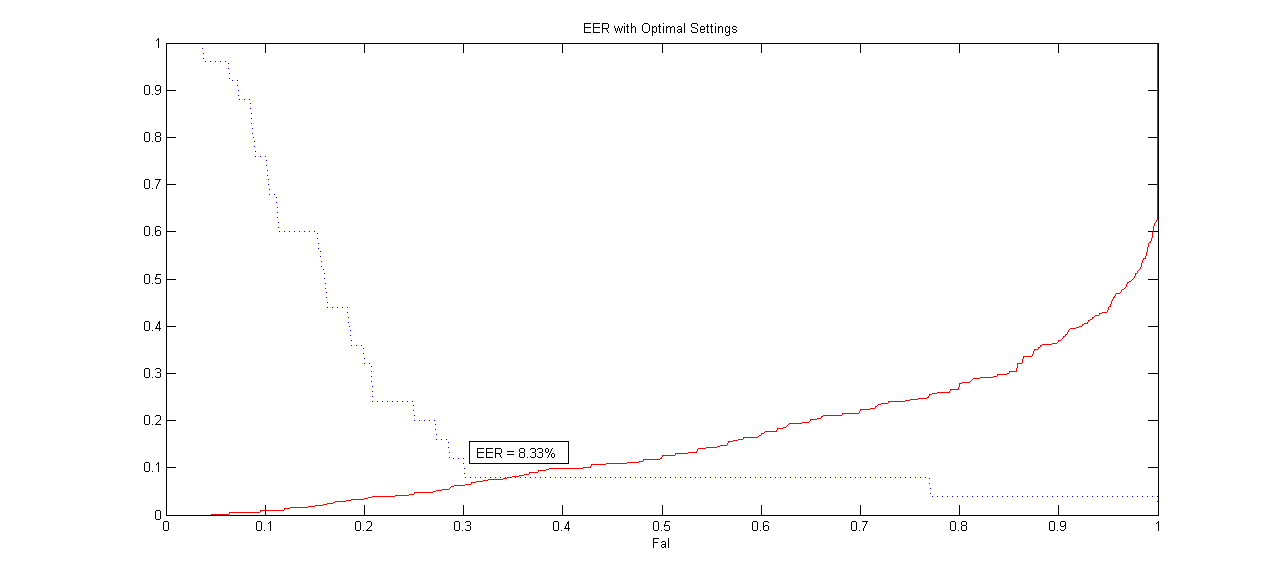
\includegraphics[width=.8\linewidth]{Optimal}
  \caption{Optimal Settings\\Single Click R = 20ms Double Click R = 185ms\\M-Value = 2.2}
  \label{fig:sfig1}
\end{subfigure}%
\begin{subfigure}{.5\textwidth}
  \centering
  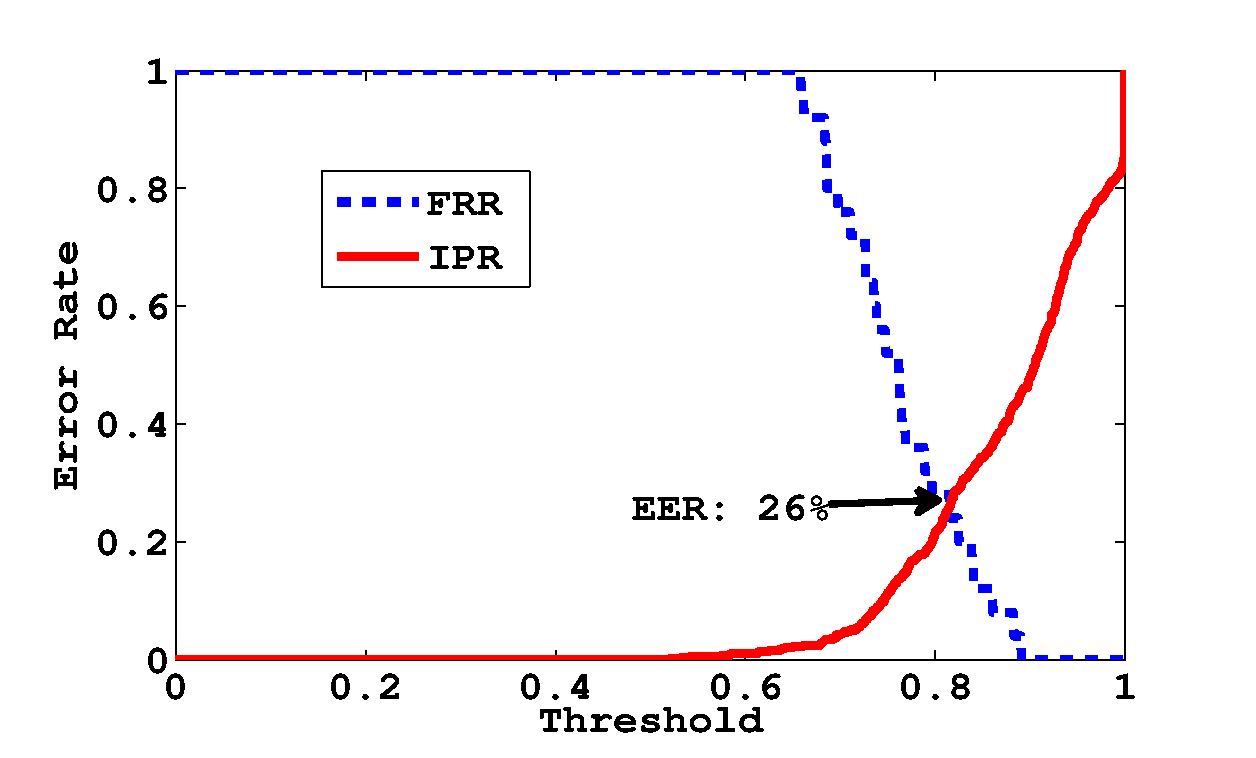
\includegraphics[width=.8\linewidth]{7M}
  \caption{Single Click R = 35ms Double Click R = 195ms\\M-Value = 0.7}
  \label{fig:sfig2}
\end{subfigure}
\begin{subfigure}{.5\textwidth}
  \centering
  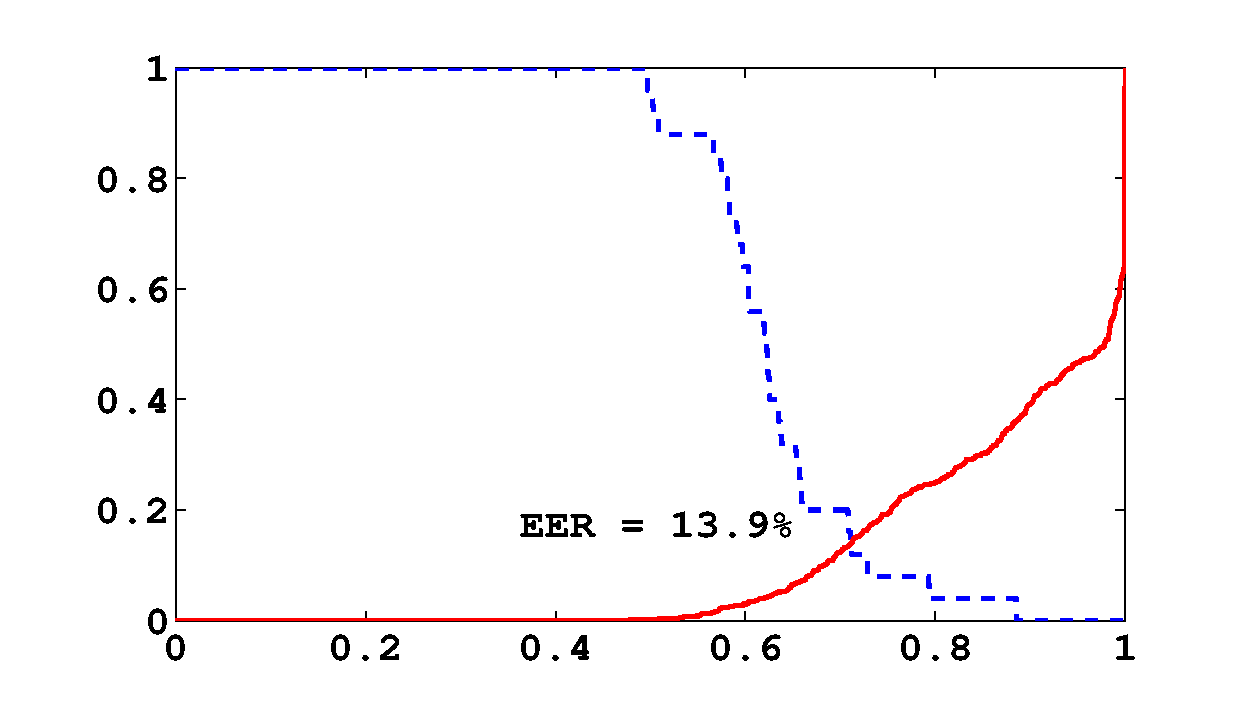
\includegraphics[width=.8\linewidth]{M1}
  \caption{Single Click R = 20ms Double Click R = 180ms\\M-Value = 1}
  \label{fig:sfig3}
\end{subfigure}%
\begin{subfigure}{.5\textwidth}
  \centering
  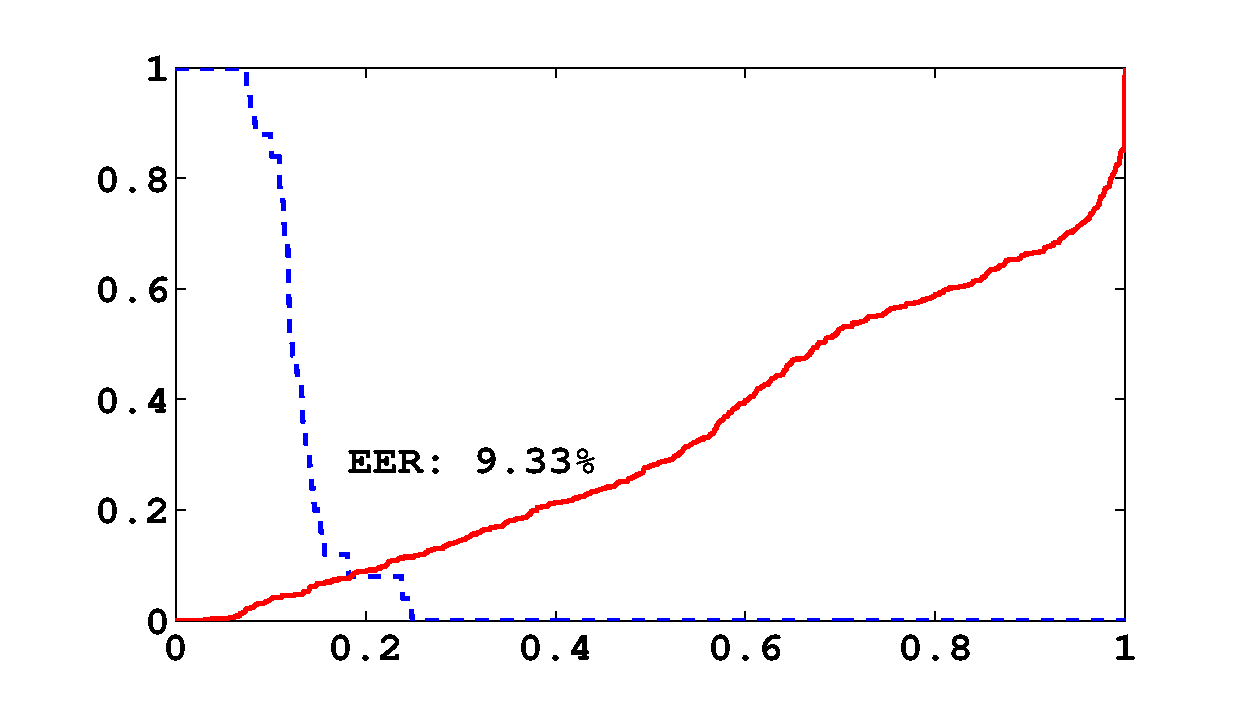
\includegraphics[width=.8\linewidth]{19M}
  \caption{Single Click R = 30ms Double Click R = 190m\\ M-Value = 1.9}
  \label{fig:sfig4}
\end{subfigure}
\caption{Plots of the False Rejection Rate and the False Acceptance Rate for four different parameter settings. The point at which the FRR and FAR intersect is the Equal Error Rate. }
\label{fig:fig}
\end{figure*}

\begin{figure*}[b!]
\begin{subfigure}{.5\textwidth}
  \centering
  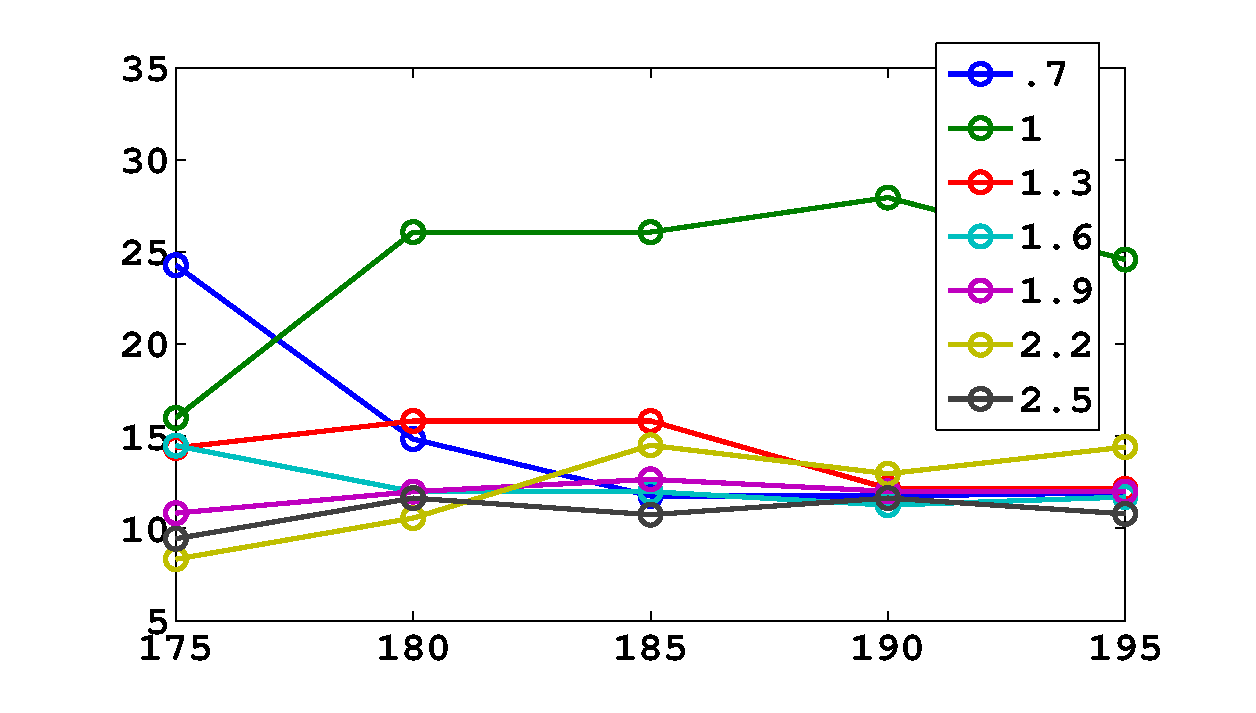
\includegraphics[width=.8\linewidth]{15.eps}
  \caption{Single Click R = 15ms \\Local Max = 24.29\% Local Min = 8.33\% \\Local Average = 14.34\% Local STD = 5.08\%}
\centering
  \label{fig:sfig1}
\end{subfigure}%
\begin{subfigure}{.5\textwidth}
  \centering
  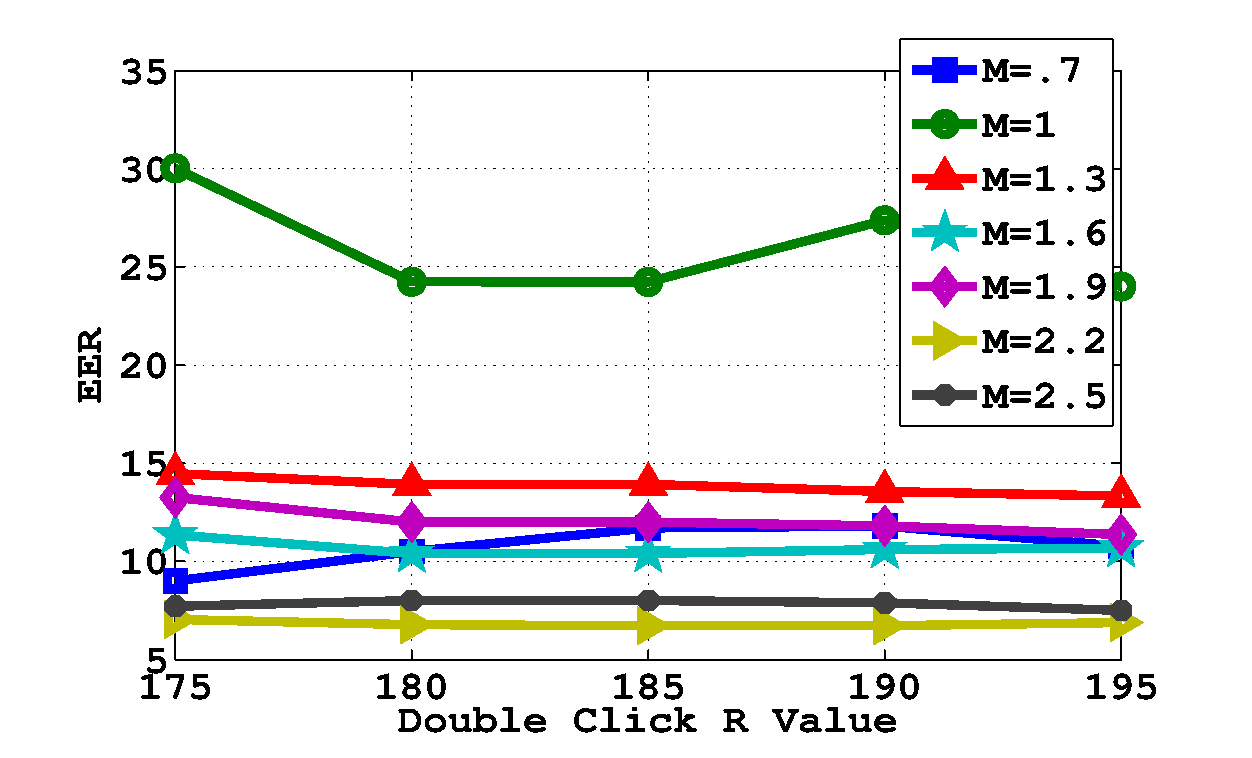
\includegraphics[width=.8\linewidth]{25.eps}
  \caption{Single Click R = 25ms \\Local Max = 30.02\% Local Min = 6.77\% \\Local Average = 12.57\% Local STD = 6.07\%}
  \label{fig:sfig2}
\end{subfigure}
\begin{subfigure}{.5\textwidth}
  \centering
  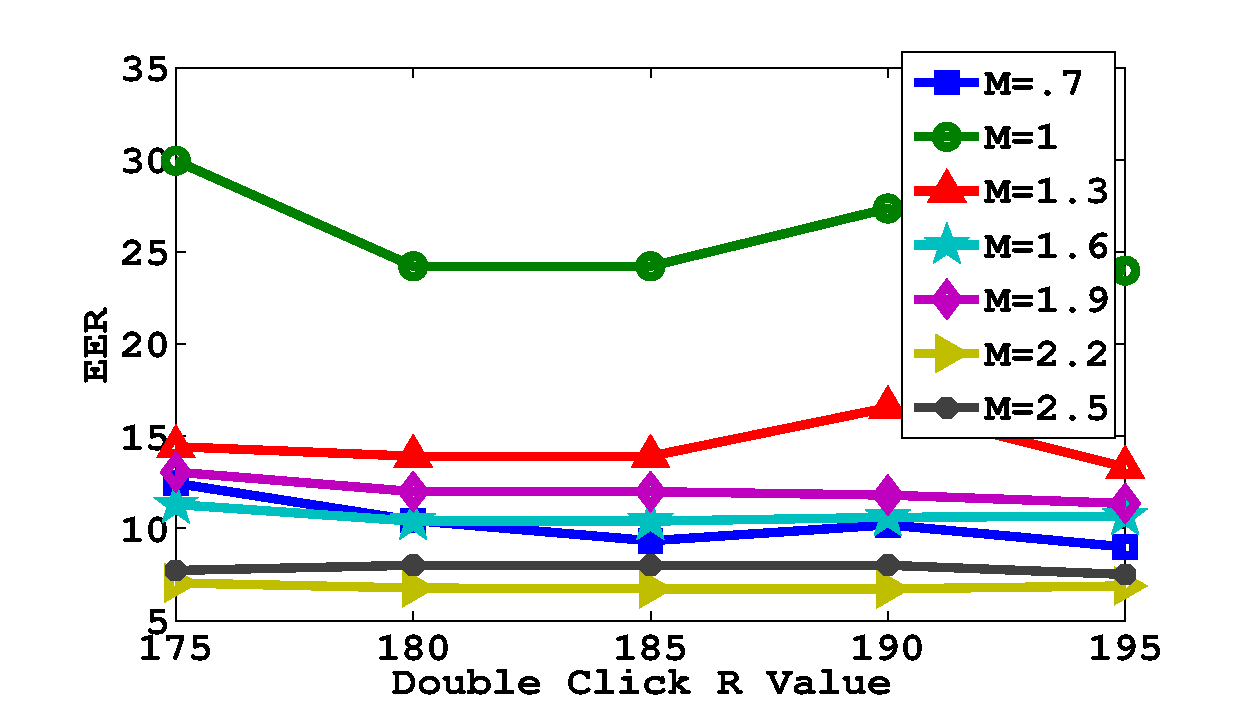
\includegraphics[width=.8\linewidth]{30.eps}
  \caption{Single Click R = 30ms \\Local Max = 29.96\% Local Min = 6.72\% \\Local Average = 12.58\% Local STD = 6.13\%}
  \label{fig:sfig3}
\end{subfigure}%
\begin{subfigure}{.5\textwidth}
  \centering
  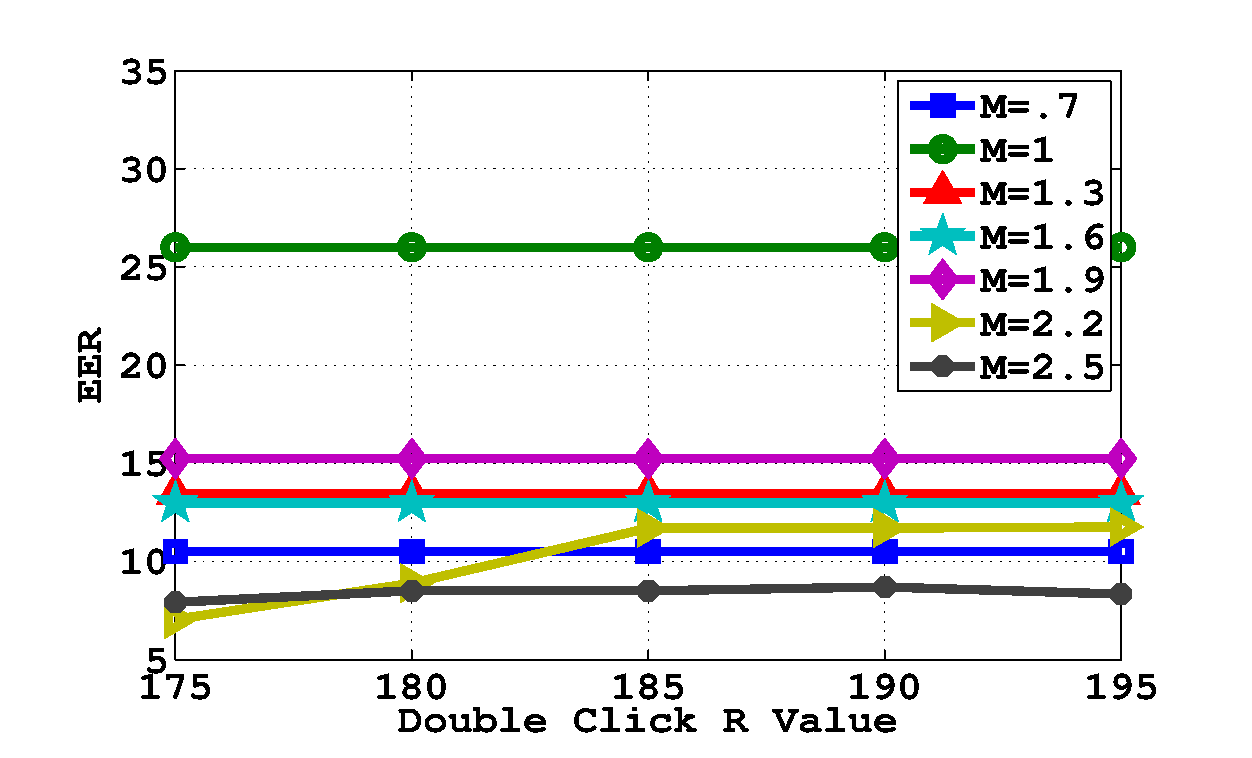
\includegraphics[width=.8\linewidth]{35.eps}
  \caption{Single Click R = 35ms \\Local Max = 26\% Local Min = 7.04\%\\Local Average = 13.82\% Local STD = 5.54\%}
  \label{fig:sfig4}
\end{subfigure}
\caption{Scatter plots of EER over the ranges of the parameter values we chose. The X-axis is Double Click R-Values, the Y-axis is the EER. Each plot is a separate Single Click R value. \\Global Max = 30.02\% Global Min = 6.72\% Global Average = 13.19\% Global STD = 5.77\%}
\label{fig:fig}
\end{figure*}


\section{Conclusion}

Our comprehensive experiment which comprises X thousands verification attempts carried over 45 users, shows the effectiveness of our method. On average, the EER we found was 13.42\%. The lowest EER was found to be 6.72\%. In future, we want to test our method on more user samples. To improve accuracy even further, we want to set the parameter values (R and M) for each users separately instead of adopting generic values. We believe that, a simple system with impressive accuracy such as ours, can easily be considered for continuously verify system users in real time.    

\section*{Acknowledgment}
We acknowledge the acknowledged acknowledgees.


\begin{thebibliography}{100} % 100 is a random guess of the total number of
%references

\bibitem{Ahmed} A. Ahmed and I. Traore, 'A New Biometric Technology Based on Mouse Dynamics', IEEE Trans. Dependable and Secure Comput., vol. 4, no. 3, pp. 165-179, 2007.
\bibitem{CS} Chao Shen, Zhongmin Cai, Xiaohong Guan, Youtian Du and R. Maxion, 'User Authentication Through Mouse Dynamics', IEEE Trans.Inform.Forensic Secur., vol. 8, no. 1, pp. 16-30, 2013.
\bibitem{HJ} H. Jahankhani, D. Palmer-Brown and K. Revett, 'A Survey of User Authentication Based on Mouse Dynamics', Global E-Security. Berlin, Heidelberg: Springer-Verlag Berlin Heidelberg, 2008, pp. 210-219.
\bibitem{Jor} Z. Jorgensen and T. Yu, 'On mouse dynamics as a behavioral biometric for authentication', Proceedings of the 6th ACM Symposium on Information, Computer and Communications Security - ASIACCS '11, pp. 476-482, 2011.
\bibitem{Nak}Y. Nakkabi, I. Traore and A. Ahmed, 'Improving Mouse Dynamics Biometric Performance Using Variance Reduction via Extractors With Separate Features', IEEE Trans. Syst., Man, Cybern. A, vol. 40, no. 6, pp. 1345-1353, 2010.
\bibitem{Pus}M. Pusara and C. Brodley, 'User re-authentication via mouse movements', Proceedings of the 2004 ACM workshop on Visualization and data mining for computer security - VizSEC/DMSEC '04, 2004.
\bibitem{Sch}D. Schulz, 'Mouse Curve Biometrics', 2006 Biometrics Symposium: Special Session on Research at the Biometric Consortium Conference, 2006.
\bibitem{She}C. Shen, Z. Cai, X. Guan, H. Sha and J. Du, 'Feature Analysis of Mouse Dynamics in Identity Authentication and Monitoring', 2009 IEEE International Conference on Communications, 2009.
\bibitem{Syu}A. Syukri, E. Okamoto and M. Mambo, 'A user identification system using signature written with mouse', Information Security and Privacy, pp. 403-414, 1998.
\bibitem{Zhe}N. Zheng, A. Paloski and H. Wang, 'An efficient user verification system via mouse movements', Proceedings of the 18th ACM conference on Computer and communications security - CCS '11, pp. 139-150, 2011.

\end{thebibliography}


\end{document}